% Use only LaTeX2e, calling the article.cls class and 12-point type.

\documentclass[12pt]{article}


% Users of the {thebibliography} environment or BibTeX should use the
% scicite.sty package, downloadable from *Science* at
% www.sciencemag.org/about/authors/prep/TeX_help/ .
% This package should properly format in-text
% reference calls and reference-list numbers.

\usepackage{scicite}

% Use times if you have the font installed; otherwise, comment out the
% following line.

\usepackage{times}
\usepackage{graphicx}
\usepackage{caption} % removes colon after empty caption


% The preamble here sets up a lot of new/revised commands and
% environments.  It's annoying, but please do *not* try to strip these
% out into a separate .sty file (which could lead to the loss of some
% information when we convert the file to other formats).  Instead, keep
% them in the preamble of your main LaTeX source file.


% The following parameters seem to provide a reasonable page setup.
\topmargin 0.0cm
\oddsidemargin 0.2cm
\textwidth 16cm 
\textheight 21cm
\footskip 1.0cm


%The next command sets up an environment for the abstract to your paper.

\newenvironment{sciabstract}{%
\begin{quote} \bf}
{\end{quote}}


% If your reference list includes text notes as well as references,
% include the following line; otherwise, comment it out.

\renewcommand\refname{References and Notes}

% The following lines set up an environment for the last note in the
% reference list, which commonly includes acknowledgments of funding,
% help, etc.  It's intended for users of BibTeX or the {thebibliography}
% environment.  Users who ae hand-coding their references at the end
% using a list environment such as {enumerate} can simply add another
% item at the end, and it will be numbered automatically.

\newcounter{lastnote}
\newenvironment{scilastnote}{%
\setcounter{lastnote}{\value{enumiv}}%
\addtocounter{lastnote}{+1}%
\begin{list}%
{\arabic{lastnote}.}
{\setlength{\leftmargin}{.22in}}
{\setlength{\labelsep}{.5em}}}
{\end{list}}


% Include your paper's title here

\title{The length of words reflects their conceptual complexity}


% Place the author information here.  Please hand-code the contact
% information and notecalls; do *not* use \footnote commands.  Let the
% author contact information appear immediately below the author names
% as shown.  We would also prefer that you don't change the type-size
% settings shown here.

\author
{Molly Lewis and Michael C. Frank\\
\\
\normalsize{Psychology Department, Stanford University,}\\
\normalsize{450 Serra Mall, Stanford, CA 94305, USA}\\
\\
\normalsize{$^\ast$To whom correspondence should be addressed; E-mail: mll@stanford.edu.}
}


% Include the date command, but leave its argument blank.

\date{}



%%%%%%%%%%%%%%%%% END OF PREAMBLE %%%%%%%%%%%%%%%%
\begin{document} 

% Double-space the manuscript.
\baselineskip24pt

% Make the title.
\maketitle 

% Place your abstract within the special {sciabstract} environment.

\begin{sciabstract}
 Are the forms of words systematically related to their meaning? The �arbitrariness of the sign� has long been a foundational part of our understanding of human language\cite{saussure, hockett1960}. Theories of communication predict a relationship between form and meaning, however: longer descriptions should convey more complex meanings\cite{horn1984,jaeger2006}. Here we show that the lexicons of human languages reflect this relationship between linguistic and cognitive complexity. We asked participants to rate the conceptual complexity of word meanings and found that their judgements correlated highly with word length across 80 languages, even controlling for frequency and concreteness. This relationship is productively encoded in the minds of speakers, as well: Adults and children both mapped longer words to more complex meanings, and more complex meanings to longer words, in comprehension and production tasks and across a wide range of stimuli. In addition, explicit judgments of complexity were highly correlated with an implicit measure of study time in a memory task, suggesting that complexity is directly related to basic cognitive processes. These results point to a general regularity in the design of lexicons and suggests the importance of cognitive constraints on language evolution\cite{christiansen2008,lieberman2007}.
 \end{sciabstract}


%Letters no more than 4 pages, of Nature. A typical Letter to Nature contains about 1,500 words of text (excluding the first paragraph of Letters, figure legends, reference list and the methods section if applicable) and four small display items (figures and/or tables) with brief legends. A composite figure (with several panels) usually needs to take about half a page, equivalent to about 600 words, in order for all the elements to be visible (see section 5.9 for instructions on sizing figures).

% intro
Human languages universally contain sequences of sounds --- words --- that are associated with particular meanings. A foundational part of our understanding of human language is that these associations are arbitrary \cite{saussure,hockett1960}. This assumption is supported by a superficial survey of word forms across languages: different languages use different words to refer to similar meanings.  However, several theories of communication predict a systematicity in these mappings\cite{horn1984,jaeger2006}. They predict that longer utterances should be associated with more complex meanings. Here we address whether this bias is present in language at the level of words. We first examine whether speakers have a lexical complexity bias that is productive by asking how speakers interpret novel words. Given evidence for a productive complexity bias in words, we then ask whether this systematicity is encoded in the lexicon of 80 languages. 

[a paragraph here about how theories of communication predict a complexity bias?]

%communicative pressures should lead to a complexity bias that operates at the moment of language interpretation.

%Uniform information theory predicts that  speakers should try to maintain a constant rate of information transfer across the speech stream. A straight forward consequence of this prediction is that speakers should try to use longer linguistic forms to refer to less predictable meanings.
%More specifically, they predict that communicative pressures should lead to a complexity bias that op- erates at the moment of language interpretation.

%Uniform information theory predicts that  speakers should try to maintain a constant rate of information transfer across the speech stream. A straight forward consequence of this prediction is that speakers should try to use longer linguistic forms to refer to less predictable meanings. 

\begin{figure}[t]
\begin{center}
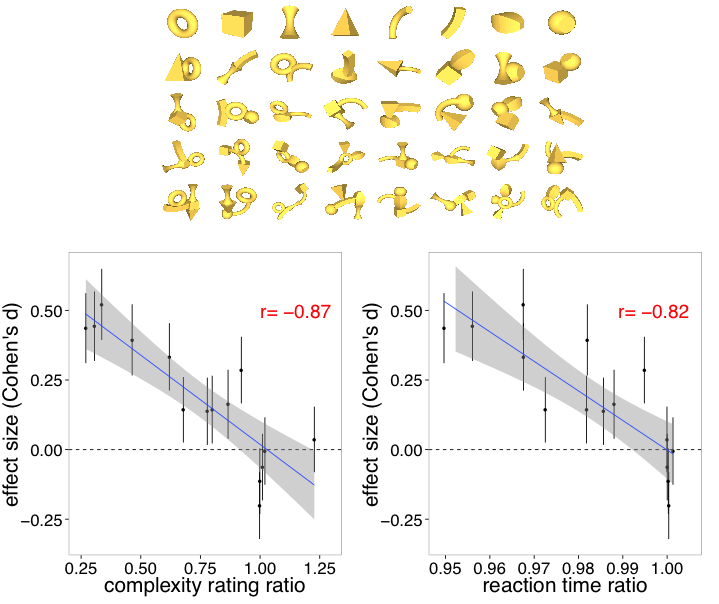
\includegraphics[scale = .5]{figs/geons_cropped.png}
\caption{}
\end{center}
\label{fig:geons}
\end{figure}

\begin{figure}[t]
\begin{center}
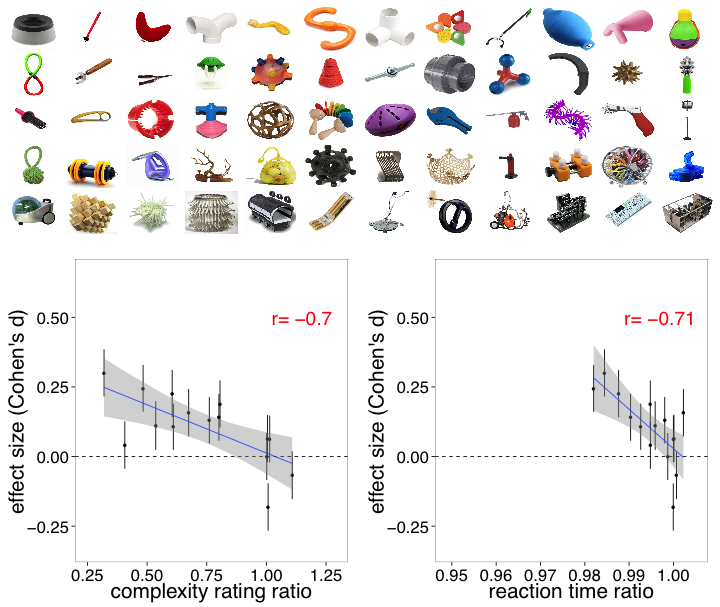
\includegraphics[scale = .5]{figs/real_objs_cropped.png}
\caption{}
\end{center}
\label{fig:real_objs}
\end{figure}


%We began by asking how speakers interpreted the meaning of novel words of varying lengths
We began by asking whether speakers are biased to interpret a long novel word as being more likely to refer to a more complex novel referent. We presented 750 adult English speakers with a novel word and two possible alternative referents. Participants were asked to select the intended referent from the two alternatives. The possible referents were novel artificial objects of varying complexity. We manipulated complexity by varying the number of parts the object  contained (1-5 parts;  Fig.\ 1a). This manipulation was highly correlated with speakers' explicit judgements of object complexity ($r = .93$, $p<.01$). We tested every unique combination of complexity of the object alternatives (1 vs.\ 2 parts, 1 vs.\ 3 parts, 1 vs.\ 4 parts, etc.). Word length was manipulated across trials to have either 2 or 4 syllables. %Each participant completed 8 trials total, with four short words and four long words.

For each object complexity condition, we calculated the relative bias between the short and long word conditions  to select the more complex referent (effect size). Figure 1b shows the effect size for each complexity condition plotted as a function of the ratio of the explicit complexity judgments of the object alternatives. Effect size and complexity judgment ratio were highly negatively correlated ($r = .87$, $p<.01$), suggesting that participants were more likely to select the more complex referent when they were presented with a long word compared to a short word. Furthermore, this judgement was sensitive to the relative complexity of the two alternatives: the complexity bias was larger when there was a larger discrepancy in  complexity between the two referent alternatives.

Next we asked whether this bias extended to more naturalistic objects. We recruited 60 participants to rate the complexity of 60 novel, real objects. This judgement had a reliability of\  $.93$  in a second sample of 60 participants. Based on these complexity ratings, we divided the objects into quintiles (Fig.\ 2a), and used these as stimuli in a reference task identical in design to that of the artificial objects. As with the artificial objects,  effect size was highly negatively correlated with the complexity judgment ratio between the referent alternatives ($N=1500$; $r = .70$, $p<.01$, Fig. 2b). We also found the same bias in language production: participants were more likely to produce a longer novel label or a longer description of objects that were rated as more complex. [mention the result with kids here?]

These experiments suggest that speakers' explicit complexity judgements  are related to the length of novel words. We reasoned that if complexity is related to a basic cognitive process, we should be able to measure the complexity of stimuli in an implicit task. In particular, we predicted that a stimulus that contains more information should take more time to process \cite{alvarez2004capacity}. To test this prediction, we  measured participants' reaction time to objects in a memory task. Participants were told they would be presented with some pictures of objects, and then their memory for those objects would be tested. In the training phase, each participant viewed half of the objects in the stimulus set one at a time (20 for the artificial objects and 30 for the novel real objects). In the test phase, participants were asked to indicate whether an object was old or new for each object in the stimulus set (40 for the artificial objects and 60 for the novel real objects). Critically, the training phase was self-paced, such that participants were allowed to study each object for as much time as they wanted. We recruited 250 participants to complete the task with the artificial objects and 500 participants to complete the task with the novel real objects.

We used the mean study time for each object as a measure of the complexity of the object. This measure was highly correlated with the explicit complexity norms for both the artificial objects ($r = .89$, $p<.01$) and the novel real objects ($r = .54$, $p<.01$). As for the complexity judgements, we calculated the ratio in reaction time between the two object alternatives for each reference condition. The reaction time ratio was negatively correlated with effect size for both the artificial objects ($r = .82$, $p<.01$; Fig 1c) and the novel real objects ($r = .71$, $p<.01$; Fig 2c), suggesting that the reference judgement is supported by a basic cognitive process related to the complexity of the stimulus.

These experiments point to a productive complexity bias in language: Words that are longer tend to be associated with meanings that are more complex in terms of both explicit and implicit judgements. Given the presence of a productive complexity bias, we predicted that this bias might also be encoded in the structure of natural languages. To test this, we asked 250 participants to rate the complexity of the meaning of 499 English words. These judgements were positively correlated with word length in terms of syllables ($r = .63$, $p<.01$), phonemes ($r = .66$, $p<.01$), and morphemes ($r = .43$, $p<.01$). This relationship also held for the subset of mono-morphemic words in our sample ($n=387$; syllables: $r =.46$, $p<.01$; phonemes: $r = .53$, $p<.01$), and for the subset of open class words in our sample ($n=453$; syllables: $r =.62$, $p<.01$; phonemes: $r = .66$, $p<.01$; morphemes: $r = .43$, $p<.01$). Importantly, these relationships remained reliable after controlling for log spoken frequency, concreteness, imaginability and familiarity. This suggests that the bias to map longer words to more complex meanings with novel words is also reflected in the structure of natural language.
%Each participant rated the complexity of the meaning of a random subset of 30 words using a 7-point Likert scale. 
\begin{figure}[t]
\begin{center}

\includegraphics[scale = .55]{figs/xling.pdf}
\caption{}
\end{center}
\label{fig:real_objs}
\end{figure}


If the complexity bias relies on a universal cognitive process, it should generalize to lexicons beyond English. We explored this prediction in 79 additional languages, using Google Translate to translate our set of 499 words.  Native speakers checked the accuracy of these translations for 12 of the 79 language, finding an accuracy of .92 within this sample. 

In the analysis of the cross-linguistic corpus, we used number of characters as the metric of length because it was easily available across languages. For each language, we calculated the correlation between word length in terms of number of characters and mean complexity rating. All of the languages showed a positive correlation between length and complexity rating (Fig.\ 3). The grand mean correlation across language was .34 (monomorphic: $r = .23$; open-class: $r = .31$). Partialling out the effect of log spoken frequency, the grand mean correlation across languages was .22. In addition, word lengths across languages were highly correlated with each other ($r = .31$). 



Finally, we examined whether the lengths of real words are related to the complexity of known meanings measured in a reaction time task.

[some sort of brief conclusion]

%\paragraph*{Tables}
\paragraph*{Figure Legends}

Figure 1: [These plots needs some work]

Figure 2: 

Figure 3: [fix key] Squares: open class words; Triangles: partialling out frequency; Circles: Mono-morphemic words 
\paragraph*{Methods}
\paragraph*{References}
\paragraph*{Acknowledgements}
\paragraph*{Author Contributions}
\paragraph*{Author Information}


\bibliography{biblibrary}

\bibliographystyle{Science}



% Following is a new environment, {scilastnote}, that's defined in the
% preamble and that allows authors to add a reference at the end of the
% list that's not signaled in the text; such references are used in
% *Science* for acknowledgments of funding, help, etc.



% For your review copy (i.e., the file you initially send in for
% evaluation), you can use the {figure} environment and the
% \includegraphics command to stream your figures into the text, placing
% all figures at the end.  For the final, revised manuscript for
% acceptance and production, however, PostScript or other graphics
% should not be streamed into your compliled file.  Instead, set
% captions as simple paragraphs (with a \noindent tag), setting them
% off from the rest of the text with a \clearpage as shown  below, and
% submit figures as separate files according to the Art Department's
% instructions.


\clearpage



\end{document}



